\documentclass[12pt]{article}
\usepackage[utf8]{inputenc}
\usepackage{hyperref}
\usepackage{listings}
\usepackage{xcolor}
\usepackage{geometry}
\usepackage{graphicx} % For including graphics
\usepackage{listings-solidity}  % Include Solidity highlighting
\usepackage{minted} % For advanced code listings

% Define a custom minted style (optional)
\usemintedstyle{colorful} % You can choose from various styles like 'monokai', 'tango', 'colorful', etc.

% Custom color setup
\definecolor{bashtextcolor}{RGB}{0, 0, 0} % Define black color

% Define a new command for inline code using minted
\newcommand{\codeinline}[1]{\mintinline{text}{#1}}

\geometry{a4paper, margin=1in}

\title{Smart Contracts Exercise 03: \\ ERC-20 CTU Token}
\author{}
\date{}

% Define a new command for inline code with a dark background
\newcommand{\codeblack}[1]{%
  \texttt{\colorbox{black!7}{\textcolor{black}{#1}}}%
}

% Define a new command for inline code with a dark background
\newcommand{\codegrey}[1]{%
  \texttt{\colorbox{black!4}{\textcolor{black}{#1}}}%
}

% Define custom colors (optional)
\definecolor{myURLColor}{RGB}{0, 102, 204} % Example: A shade of blue

\hypersetup{
    colorlinks=true,        % Enable colored links
    linkcolor=blue,         % Color for internal links (e.g., \ref, \cite)
    citecolor=blue,         % Color for citations
    filecolor=magenta,      % Color for file links
    urlcolor=myURLColor     % Color for external URLs
}

% Define a style for code listings
\lstdefinestyle{mystyle}{
    backgroundcolor=\color{lightgray!20},   
    commentstyle=\color{green!50!black},
    keywordstyle=\color{blue},
    numberstyle=\tiny\color{gray},
    stringstyle=\color{red},
    basicstyle=\ttfamily\footnotesize,
    breakatwhitespace=false,         
    breaklines=true,                 
    captionpos=b,                    
    keepspaces=true,                 
    numbers=left,                    
    numbersep=5pt,                  
    showspaces=false,                
    showstringspaces=false,
    showtabs=false,                  
    tabsize=2
}

\lstset{style=mystyle}
% Adding package for header and footer
\usepackage{fancyhdr}
\pagestyle{fancy}

% Define header and footer
\fancyhf{} % Clear current settings
\fancyhead[L]{Smart Contracts Exercise 03} % Left header
\fancyhead[R]{\thepage} % Right header with page number

\renewcommand{\headrulewidth}{0.4pt} % Line below header
% \renewcommand{\footrulewidth}{0.4pt} % Line above footer

\begin{document}

\maketitle
\section{Introduction}

Tokens in the Ethereum ecosystem are smart contracts that implement a standardized interface. They are designed to represent various assets digitaly. These assets can range from financial instruments like company shares and stablecoins (e.g., USDC, DAI) to governance tokens that allow holders to vote on decisions in decentralized projects (e.g., Uniswap's UNI). Tokens can also enable artists to tokenize their works and sell them as unique digital items (NFTs), represent collectibles in games, or are used for digital identity or access to services. Depending on the use case, there are different types of tokens, each serving distinct purposes. Below are three common types of tokens:

\begin{enumerate}
  \item \textbf{Fungible Tokens}

  Fungible tokens \href{https://eips.ethereum.org/EIPS/eip-20}{(\textit{ERC-20 Tokens})} are interchangeable and have exactly the same value. Each unit of a fungible token is identical to another unit. Examples are cryptocurrencies, utility tokens or governance tokens.

    \begin{figure}[h!]
      \centering
      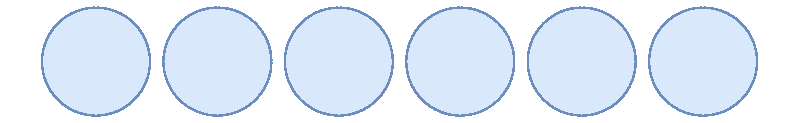
\includegraphics[width=0.5\textwidth]{fungible-tokens.pdf}
      \caption{Fungible Tokens}
      \label{fig:fungible-tokens}
    \end{figure}

    \item \textbf{Non-Fungible Tokens (NFTs)}

    Non-fungible tokens \href{https://eips.ethereum.org/EIPS/eip-721}{(\textit{ERC-721 Tokens})} are unique and cannot be exchanged on a one-to-one basis. They are used to represent ownership of unique items such as digital art, collectibles, and real estate. Each token is uniquely identifiable by an ID.

    \begin{figure}[h!]
      \centering
      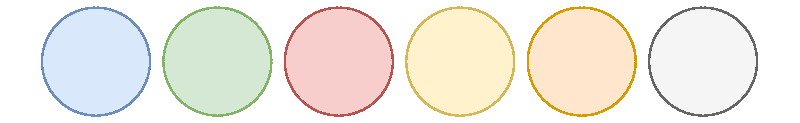
\includegraphics[width=0.5\textwidth]{non-fungible-tokens.pdf}
      \caption{Non-Fungible Tokens}
      \label{fig:non-fungible-tokens}
    \end{figure}

    \item \textbf{Multi-Tokens}

    Multi-tokens \href{https://eips.ethereum.org/EIPS/eip-1155}{(\textit{ERC-1155 Tokens})} combine the properties of both fungible and non-fungible tokens. They allow for the creation of multiple token types within a single contract, providing flexibility for various use cases.

    \begin{figure}[h!]
      \centering
      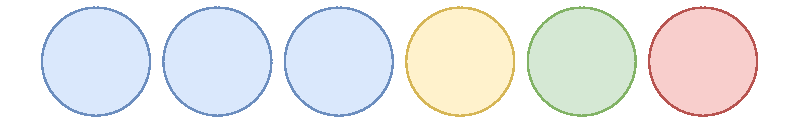
\includegraphics[width=0.5\textwidth]{multi-token.pdf}
      \caption{Multi-Tokens}
      \label{fig:multi-token}
    \end{figure}
  \end{enumerate}

In this exercise, you'll create your own ERC-20 token contract following the specified standard, and then attempt to hack it. For more information about tokens, check out this animated video: \href{https://www.youtube.com/watch?v=Xdkkux6OxfM}{What Are NFTs and How Can They Be Used in Decentralized Finance?} You'll also work with your own NFTs in future exercises.

\subsection*{Project Setup}

You have two options for working with this exercise. Using docker container or local installation. Choose the one that best fits your preferences.

\subsection{Using Docker with VS Code}

This option uses Docker to create a development environment with all the necessary tools and dependencies pre-installed.

\subsubsection*{Prerequisites:}

\begin{itemize}
    \item \textbf{\href{https://www.docker.com/products/docker-desktop}{Docker}} - A platform for developing, shipping, and running applications in containers.
    \item \textbf{\href{https://code.visualstudio.com/}{Visual Studio Code}} - A lightweight but powerful source code editor.
    \item \textbf{\href{https://marketplace.visualstudio.com/items?itemName=ms-vscode-remote.remote-containers}{Dev Containers}} - An extension to VS Code that lets you use a Docker container as a full-featured development environment.
\end{itemize}

\subsubsection*{Setting Up the Project:}

\begin{enumerate}
  \item Visit the following \href{https://gitlab.fel.cvut.cz/radovluk/smart-contracts-exercises/-/tree/main/03-ERC20-CTUToken/task/task-code?ref_type=heads}{GitLab repository} and clone it to your local machine.
  \item Open the repository folder in VS Code.
  \item When prompted, click "Reopen in Container" or use the command palette (F1) and run \codegrey{Dev Containers: Reopen in Container}.
\end{enumerate}

\subsection{Local Setup}

If you prefer working directly on your machine without Docker, you can set up the development environment locally.

\subsubsection*{Prerequisites}
\begin{itemize}
    \item \textbf{Node.js} - \url{https://nodejs.org/en/} - An open-source, cross-platform, back-end JavaScript runtime environment that runs on the V8 engine and executes JavaScript code outside a web browser.
    \item \textbf{NPM}: Node Package Manager, which comes with Node.js.
\end{itemize}

\noindent
Open your terminal and run the following commands to verify the installations:

\begin{minted}[bgcolor=gray!5, fontsize=\footnotesize]{bash}
$ node -v
$ npm -v
\end{minted}

Both commands should return the installed version numbers of Node.js and NPM respectively. Node.js provides the runtime environment required to execute JavaScript-based tools like Hardhat, while NPM is used to manage the packages and dependencies needed for development.

\subsubsection*{Setting Up the Project}

\begin{enumerate}
    \item Visit the following \href{https://gitlab.fel.cvut.cz/radovluk/smart-contracts-exercises/-/tree/main/03-ERC20-CTUToken/task/task-code?ref_type=heads}{GitLab repository} and clone it to your local machine.
    \item Open a terminal and navigate to the project directory.
    \item Install the project dependencies by running \codegrey{npm install}.
\end{enumerate}

\section{Specification: ERC-20 Token}

The ERC-20 standard was first proposed by Fabian Vogelsteller and Vitalik Buterin in November 2015. The token specification defines the interface that a smart contract must implement to be ERC-20 compliant. It is important to note that it \textbf{does not specify the actual implementation}. It is the most widely used standard with more than 1.5 million smart contracts on the mainnet implementing it.

\medskip
\noindent
Example functionalities ERC-20 provides:

\begin{itemize}
  \item Transfer tokens from one account to another.
  \item Get the current token balance of an account.
  \item Get the total supply of the token available on the network.
  \item Approve whether an amount of token from an account can be spent by a third-party account.
\end{itemize}

If a Smart Contract implements the following methods and events, it can be called an ERC-20 Token Contract. Once deployed, it will be responsible for keeping track of the created tokens on Ethereum. To see the full specification, visit \href{https://eips.ethereum.org/EIPS/eip-20}{EIP20 proposal}.

\subsubsection*{Methods}

\begin{lstlisting}[language=Solidity]
  function name() public view returns (string)
  function symbol() public view returns (string)
  function decimals() public view returns (uint8)
  function totalSupply() public view returns (uint256)
  function balanceOf(address _owner) public view returns (uint256 balance)
  function transfer(address _to, uint256 _value) public returns (bool success)
  function transferFrom(address _from, address _to, uint256 _value) 
    public returns (bool success)
  function approve(address _spender, uint256 _value) public returns (bool success)
  function allowance(address _owner, address _spender) 
    public view returns (uint256 remaining)  
\end{lstlisting}

\subsubsection*{Events}

\begin{lstlisting}[language=Solidity]
  event Transfer(address indexed _from, address indexed _to, uint256 _value)
  event Approval(address indexed _owner, address indexed _spender, uint256 _value)  
\end{lstlisting}

\subsection*{OpenZeppelin}

\href{https://www.openzeppelin.com/}{OpenZeppelin} provides an open-source library for secure smart contract development. It is built on a solid
foundation of community-vetted code. It is good practice to use standardized implementations like those from OpenZeppelin. Documentation about available contracts made by OpenZeppelin can be found \href{https://docs.openzeppelin.com/contracts/4.x/}{here}. The actual implementations of the contracts are available on \href{https://github.com/OpenZeppelin/openzeppelin-contracts}{GitHub}. OpenZeppelin contracts can be installed using npm and imported directly into a contract. The ERC20 implementation by OpenZeppelin is a standard recognized by the official EIP20 documentation. You can find the implementation \href{https://github.com/OpenZeppelin/openzeppelin-contracts/blob/master/contracts/token/ERC20/ERC20.sol}{here}. It is a common practice to use the ERC20 implementation by OpenZeppelin when creating ERC20 token contracts, instead of explicitly implementing the ERC20 interface inside the contract. However, for the educational purpose of this exercise, you will implement the ERC20 contract by yourself. The implementation of the CTU Token contract using OpenZeppelin can be seen in the code below.

\noindent
\begin{minipage}{\textwidth}
\begin{lstlisting}[language=Solidity]
// SPDX-License-Identifier: MIT
pragma solidity ^0.8.0;

// Import OpenZeppelin's ERC20 implementation
import "@openzeppelin/contracts/token/ERC20/ERC20.sol";

/**
 * @title CTUToken
 * @dev A custom implementation of an ERC-20 Token using OpenZeppelin's library.
 */
contract CTUToken is ERC20 {
    // Define the initial supply: 1,000,000 tokens with 18 decimal places
    uint256 private constant INITIAL_SUPPLY = 1_000_000 * 10 ** 18;

    /**
     * @dev Constructor that initializes the ERC-20 token with a name and symbol,
     * and mints the total supply to the deployer's address.
     */
    constructor() ERC20("CTU Token", "CTU") {
        // Mint the initial supply to the deployer of the contract
        _mint(msg.sender, INITIAL_SUPPLY);
    }
}
\end{lstlisting}
\end{minipage}

\section{CTU Token}

To complete the CTU Token contract and pass all the associated tests, you need to implement the required functionality in the \texttt{contracts/CTUToken.sol} file. Look for the sections marked with \#TODO comments and ensure that all the specified requirements below are met.

\subsection*{Token Details}
\begin{itemize}
  \item \textbf{Name}: Set the token name to \texttt{"CTU Token"}.
  \item \textbf{Symbol}: Set the token symbol to \texttt{"CTU"}.
  \item \textbf{Decimals}: Use \texttt{18} decimal places to align with the standard Ether denomination.
  \item \textbf{Total Supply}: Initialize the total supply to \texttt{1,000,000} tokens.
\end{itemize}

\subsection*{Events}
\begin{itemize}
  \item \textbf{Transfer Event}: Emit a \texttt{Transfer} event whenever tokens are transferred, including zero-value transfers.
  \item \textbf{Approval Event}: Implement and emit an \texttt{Approval} event when an allowance is set via the \texttt{approve} function.
\end{itemize}

\subsection*{Errors}
\begin{itemize}
  \item \textbf{TransferToZeroAddress}: Attempting to transfer to the zero address.
  \item \textbf{InsufficientBalance(uint256 requested, uint256 available)}: Account does not have enough balance.
  \item \textbf{ApproveToZeroAddress}: Attempting to approve the zero address as a spender.
  \item \textbf{TransferExceedsAllowance(uint256 requested, uint256 allowance)}: Trying to transfer an amount exceeding the current allowance.
\end{itemize}

\subsection*{State Variables}
\begin{itemize}
  \item \textbf{Balances Mapping}: Maintain a \texttt{mapping(address => uint256)} to track the token balance of each account.
  \item \textbf{Allowances Mapping}: Use a nested \texttt{mapping(address => mapping(address => uint256))} to manage allowances, enabling accounts to authorize others to spend tokens on their behalf.
\end{itemize}

\subsection*{Constructor}
\begin{itemize}
  \item Assign the entire \texttt{totalSupply} to the contract deployer's address upon deployment.
\end{itemize}

\subsection*{Core Functions}
\begin{itemize}
  \item \textbf{name()}: Return the name of the token.
  \item \textbf{symbol()}: Return the token symbol.
  \item \textbf{decimals()}: Return the number of decimal places (\texttt{18}).
  \item \textbf{totalSupply()}: Return the total supply of tokens in existence.
  \item \textbf{balanceOf(address account)}: Return the token balance of the specified account.
  \item \textbf{transfer(address to, uint256 value)}:
  \begin{itemize}
      \item Ensure the recipient address is not the zero address.
      \item Verify that the sender has a sufficient balance.
      \item Update the sender's and recipient's balances accordingly.
      \item Emit a \texttt{Transfer} event.
  \end{itemize}
  \item \textbf{approve(address spender, uint256 value)}:
  \begin{itemize}
      \item Ensure the spender address is not the zero address.
      \item Set the allowance for the spender.
      \item Emit an \texttt{Approval} event.
  \end{itemize}
  \item \textbf{allowance(address owner, address spender)}: Return the remaining number of tokens that the spender is allowed to spend on behalf of the owner.
  \item \textbf{transferFrom(address from, address to, uint256 value)}:
  \begin{itemize}
      \item Ensure neither the sender nor the recipient is the zero address.
      \item Verify that the source account has a sufficient balance.
      \item Check that the caller has enough allowance.
      \item Update the balances of the source and recipient accounts.
      \item Decrease the allowance accordingly.
      \item Emit a \texttt{Transfer} event.
  \end{itemize}
\end{itemize}

\noindent
To fulfill the exercise, you need to pass all the provided tests. You can run the tests with the following command:
\begin{minted}[bgcolor=gray!5, fontsize=\footnotesize]{bash}
  $ npx hardhat test
\end{minted}

\section{Frontrunning Attack}

Did your contract pass all the tests? Congratulations! It is now fully tested and ready for deployment to the mainnet. But is it really?

When you submit a transaction, it first enters the public mempool where anyone can see it. To get your transaction included in the blockchain, you need to pay a fee to validators. Validators typically choose transactions that offer the highest profit rather than processing them in chronological order. This means transactions submitted earlier might be included later, while those submitted more recently could be processed sooner. Note: this is a simplified explanation - we'll cover this topic more thoroughly in a future exercise about MEV.

\begin{figure}[H]
\centering
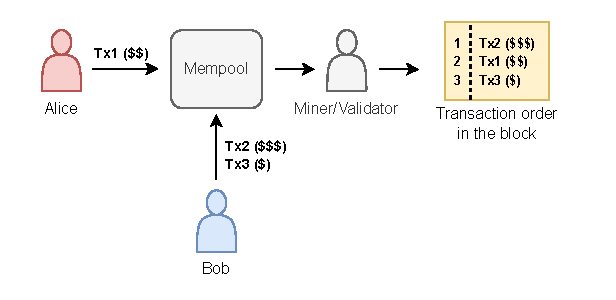
\includegraphics[width=0.75\textwidth]{sandwich.pdf}
% \caption{Frontrunning Attack}
\label{fig:frontrunning}
\end{figure}

The following table shows the attack vector for our CTU Token smart contract, where the attacker Bob manages to steal CTU tokens from Alice due to a frontrunning attack.

\begin{table}[H]
  \centering
  \begin{tabular}{|c|l|l|p{8.5cm}|}
      \hline
      \textbf{Step} & \textbf{Actor} & \textbf{Action} & \textbf{Description} \\
      \hline
      \scriptsize{1} & \scriptsize{Alice} & \scriptsize{Approve Bob} & \scriptsize{Alice approves Bob to spend 100 CTU tokens on her behalf using the \texttt{\textbf{approve}} function.} \\
      \hline
      \scriptsize{2} & \scriptsize{Bob} & \scriptsize{Monitor Mempool} & \scriptsize{Bob monitors the mempool for pending transactions, specifically looking for Alice's approval transaction.} \\
      \hline
      \scriptsize{3} & \scriptsize{Alice} & \scriptsize{Change Approval} & \scriptsize{Alice decides to change Bob's allowance from 100 CTU to 200 CTU and initiates a new \texttt{\textbf{approve}} transaction.} \\
      \hline
      \scriptsize{4} & \scriptsize{Bob} & \scriptsize{Frontrun Transaction} & \scriptsize{Upon detecting Alice's new approval transaction in the mempool, Bob quickly submits a \texttt{\textbf{transferFrom}} transaction to utilize the existing 100 CTU allowance before Alice's transaction is mined. Bob sets a higher gas price to prioritize his transaction.} \\
      \hline
      \scriptsize{5} & \scriptsize{Network} & \scriptsize{Transaction Ordering} & \scriptsize{Due to the higher gas price, Bob's \texttt{\textbf{transferFrom}} transaction is mined before Alice's new \texttt{\textbf{approve}} transaction. This allows Bob to transfer 100 CTU tokens before the allowance is updated.} \\
      \hline
      \scriptsize{6} & \scriptsize{Alice} & \scriptsize{Approval Mined} & \scriptsize{Alice's \texttt{\textbf{approve}} transaction is mined, increasing Bob's allowance to 200 CTU.} \\
      \hline
      \scriptsize{7} & \scriptsize{Bob} & \scriptsize{Exploit Increased Allowance} & \scriptsize{Bob now has an increased allowance of 200 CTU and can transfer an additional 200 CTU from Alice's account, totaling 300 CTU gained.} \\
      \hline
  \end{tabular}
  % \caption{Frontrunning Attack Scenario Between Alice and Bob}
  \label{tab:attack-scenario}
\end{table}

\medskip
\noindent
Review the file \texttt{scripts/attack.js} where this attack is implemented and understand it. Then run the attack using the command

\begin{minted}[bgcolor=gray!5, fontsize=\footnotesize]{bash}
  $ npx hardhat run scripts/attack.js --config priority.mempool.js
\end{minted}

For this attack, we use a special configuration file for Hardhat, where we set that a new block is confirmed every 500ms and transactions are selected for inclusion in the blockchain based on priority fees. In our simulation, each block contains only one transaction for simplicity. However, this does not protect against frontrunning attacks, as transactions with higher fees will simply be included in earlier blocks. 

\subsection*{Task:} Modify the CTU Token smart contract to prevent vulnerability to frontrunning attacks.

\begin{itemize}
  \item \textbf{Tip:} To display all blocks in the simulation, uncomment the last line of the main function.
  \item \textbf{Tip:} Use these functions for easier debugging: \texttt{displayState}, 
  \texttt{logTransactionDetails}, \texttt{printMempool}, \texttt{printLastBlockInfo}, \texttt{printAllBlocksInfo}.
  \item \textbf{Tip:} You might need to change the approval process completely.
\end{itemize}

\end{document}
